

\subsection{Distros}
\begin{frame}
\frametitle{Was ist eine Dist.?}
Betrieben von Community/Firmen.
Kümmern sich um: 
\begin{itemize}
 \item Pakete
 \item Änderungen/Patches
 \item Hilfe/Support
\end{itemize}
 
\end{frame}

\begin{frame}
 \frametitle{Vorkommen}

 
 \begin{itemize}
  \item Raspian/Kodi/..
  \item Android/Sailfish
  \item Alpine/TinyCore/CoreOS
  \item viele embedded Geräte mit speziell angepasstem Linux
 (wie Router, Steuergeräte, Mediengeräte)
 \end{itemize}

\end{frame}



\begin{frame}
\frametitle{Bsp. Distros}
\begin{itemize}[<+->]
\item Debian
\item Ubuntu
\item Mint
\item Arch
\item openSuse
\item RHEL/Fedora/CentOS 
\item gentoo
\item Puppy/Knoppix 

\item Kali 

\end{itemize}
\end{frame}

\subsection{Oberflächen}
\begin{frame}
\frametitle{Oberflächen}

\begin{multicols}{2}
\onslide<1->{\begin{figure}
 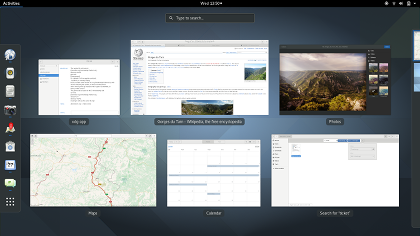
\includegraphics[width=0.45\textwidth]{resources/window-selection.png}
%\footnote{https://www.gnome.org/wp-content/uploads/2016/03/window-selection-3.20-420x236.png}
 \end{figure}
}
\onslide<2->{

\begin{figure}
 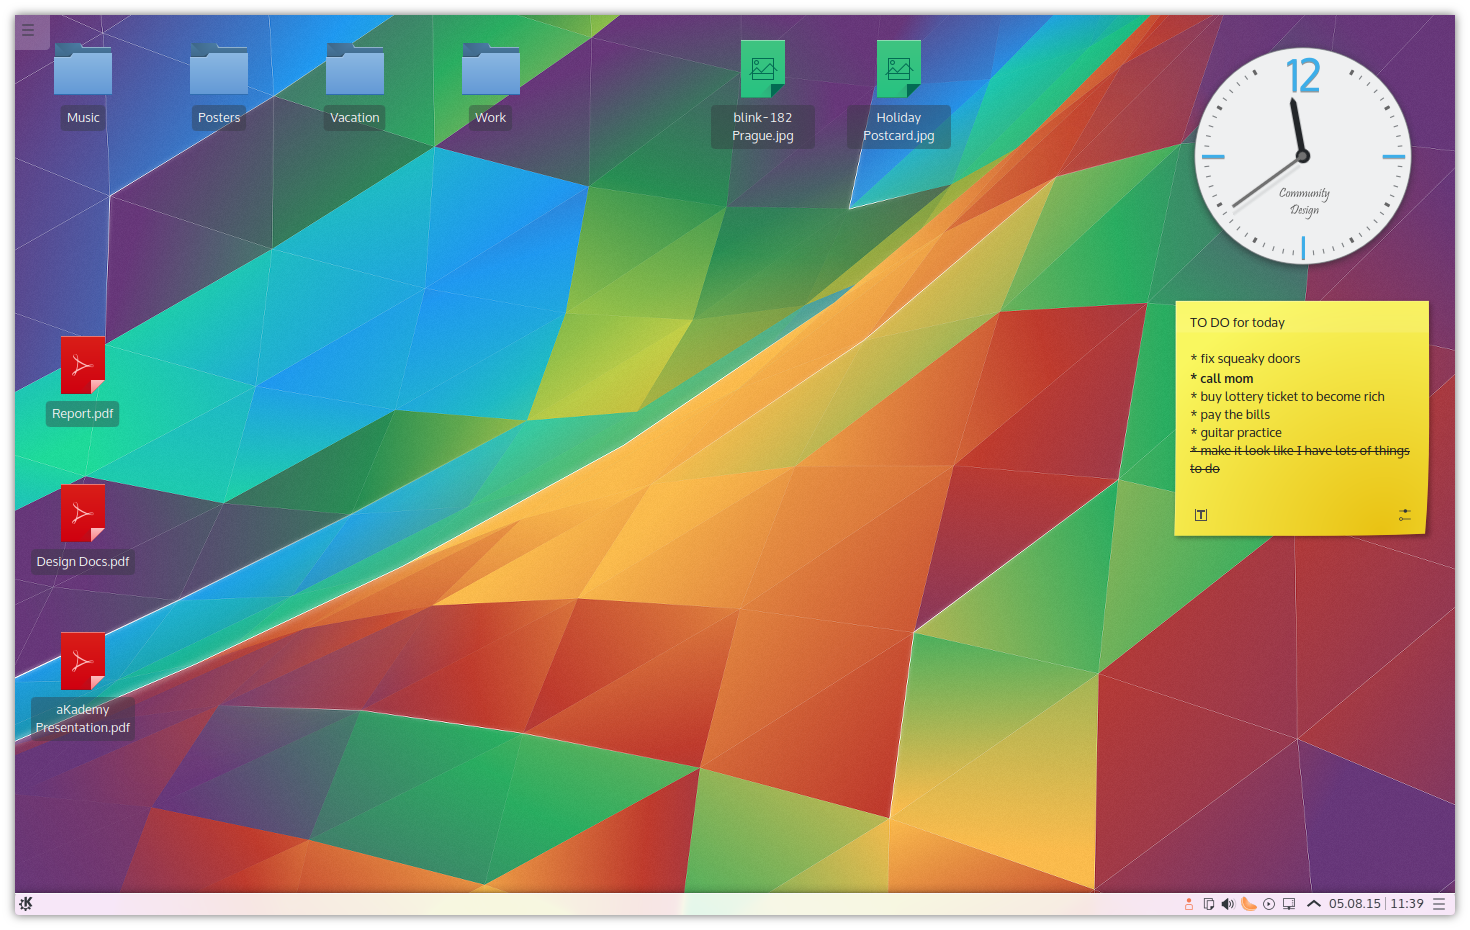
\includegraphics[width=0.45\textwidth]{resources/general-desktop.png}
\end{figure}
%\footnote{https://www.kde.org/workspaces/plasmadesktop/screenshots/general-desktop.png}
}


\only<1>{Gnome}
\only<2>{KDE: Plasma}
\only<3>{Unity (Ubuntu)}
\onslide<4>{\begin{figure}
  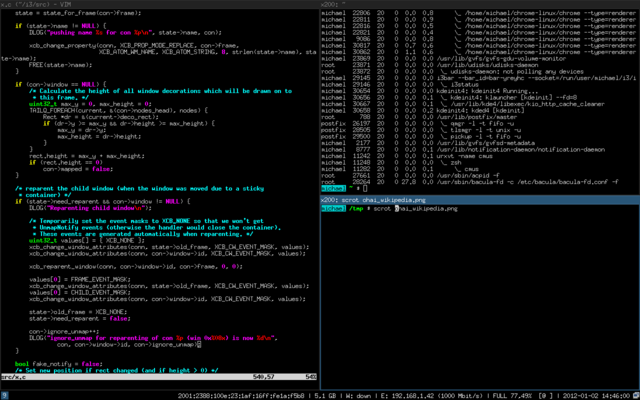
\includegraphics[width=0.45\textwidth]{resources/I3_window_manager_screenshot.png} %Nammensnennung!!
  %footnote{https://de.wikipedia.org/wiki/I3_(Fenstermanager)#/media/File:I3_window_manager_screenshot.png}
  \end{figure}
  
  \onslide<3->{\begin{figure}
  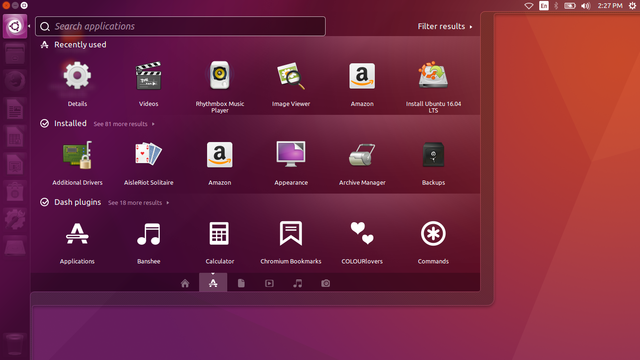
\includegraphics[width=0.45\textwidth]{resources/App_Lens_on_Ubuntu_16.png}
 %\footnote{https://en.wikipedia.org/wiki/Unity_(user_interface)#/media/File:App_Lens_on_Ubuntu_16.04LTS.png}
\end{figure}}
}

%\begin{itemize}
%\item Gnome3
%\item KDE
%\item mate
%\item Konsole
%\end{itemize}

\end{multicols}

\end{frame}


\subsection{Programme}
\begin{frame}
 \frametitle{Programme}
 \begin{tabular}{lp{5cm}}
 Kategorie& Software \\ \hline
 Internet Browser & Firefox, Waterfox, Chromium, Lynx, Opera bzw. Vivaldi, Safari, Tor Browser \\
 Office Anwendungen & LibreOffice, Kile, TeXmaker, TeXstudio, Lynx, Brasero \\
 Email Clients & Thunderbird, Icedove, Evolution \\
 Programmierung (IDEs) & Eclipse, IntelliJ, NetBeans, QtCreator, Atom, Bluefish, VI(M) \\
 
 \end{tabular}

  \end{frame}
   \begin{tabular}{lp{5cm}}

 Musik & VLC, Banshee, Rythmbox, DragonPlayer, Amarok \\
 Videos & VLC, Totem, ??? \\
 Medienproduktion & GIMP, Inkscape, Blender, Audacity, KDEnlive, AviDeMux \\
 Messenger & Gajim, Pidgin, Empathy, HexChat, WeeChat, Telegram, Matrix-Clients \\
 VoIP \& Videokonferenzen & Mumble, Ekiga, Ring, Tox \\
 Systemwerkzeuge & GParted, Wireshark, Htop, Boabab, Tor, OpenVPN, Filezilla \\
 Torrents & Transmission \\
 Synchronisation & Nextcloud, Owncloud, Seafile \\
 &DAS TERMINAL \\
 \end{tabular}
  
  \begin{frame}
   
  \end{frame}




